\documentclass[11pt]{article}
\usepackage{amsmath,amssymb,bm}
\usepackage{geometry} % For better page margins
\usepackage{graphicx}
\usepackage{hyperref}
\usepackage{tikz}
\usepackage{booktabs} % For better tables
\usepackage{multirow}
\usepackage[capitalize]{cleveref}
\usepackage{lipsum} % For placeholder text, remove in final version

\usetikzlibrary{arrows.meta, positioning, shapes, calc}
\geometry{a4paper, margin=1in}

\title{An Extended Multiplicative Extended Kalman Filter for Integrated Attitude and Wave Motion Estimation}
\author{Mikhail Grushinskiy \\ Based on the q-mekf framework by Thomas Passer}
\date{\today}

\begin{document}

\maketitle

\begin{abstract}
This paper presents an extension of the classical quaternion-based Multiplicative Extended Kalman Filter (MEKF) to simultaneously estimate the full state of a floating body: its 3D attitude, 3D velocity, 3D displacement, and an additional 3D integral-of-displacement state. This design is motivated by the problem of ocean-wave motion estimation using Inertial Measurement Units (IMUs), where accelerometer and gyroscope measurements must be fused to provide both orientation and long-period translational motion reconstruction. The method retains the structure, stability, and singularity-free properties of the MEKF for attitude estimation while systematically augmenting the state vector and covariance matrix to capture translational dynamics. A key innovation is the inclusion of a triple-integrated acceleration state ($\bm{S}$) constrained by a pseudo-measurement, which effectively mitigates the unbounded drift inherent in dead reckoning without over-constraining the velocity and displacement estimates. We provide a complete derivation of the system model, process noise, and measurement Jacobians, alongside a detailed discussion of the C++ implementation structure.
\end{abstract}

\section{Introduction}
\label{sec:introduction}
Quaternion-based Kalman filters are the cornerstone of modern attitude and heading reference systems (AHRS), providing robust orientation estimation from gyroscope, accelerometer, and magnetometer data \cite{crassidis2007survey, markley2003attitude}. The Multiplicative Extended Kalman Filter (MEKF) is a particularly well-established formulation that offers numerical stability by representing the attitude error as a minimal, 3-parameter perturbation (small Euler angles) applied multiplicatively to a reference quaternion, thus avoiding the singularities associated with direct Euler angle parameterization.

For applications such as ocean wave energy converter control, marine vessel dynamics monitoring, or buoy motion analysis, estimating orientation alone is insufficient. The primary quantity of interest is often the translational displacement caused by wave action. While accelerometers measure proper acceleration, integrating this data to obtain velocity and position is notoriously prone to drift due to sensor noise and bias. Standard double-integration approaches lead to unbounded error growth, making them unusable for long-term tracking.

To address this challenge, we propose an extended MEKF, denoted as \texttt{Kalman3D\_Wave}, that augments the classical MEKF state vector with translational quantities (velocity $\bm{v}$ and displacement $\bm{p}$) and introduces a novel third integral state ($\bm{S}$). This integral state is subjected to a zero pseudo-measurement, providing a soft statistical constraint that counteracts drift while allowing the filter to faithfully track the wave-induced motion. This approach leverages the filter's inherent understanding of uncertainty to distinguish between legitimate low-frequency motion and spurious drift.

\section{Theoretical Background}
\label{sec:theory}

\subsection{Standard Quaternion MEKF}
The standard MEKF maintains two primary quantities:
\begin{itemize}
    \item A \textbf{reference quaternion} $\bm{q}$, which is a non-minimal 4-parameter representation of the current best estimate of the attitude.
    \item An \textbf{error-state vector} $\delta \bm{x} \in \mathbb{R}^{n}$, which contains a minimal representation of the error. For attitude, this is $\delta \bm{\theta} \in \mathbb{R}^3$, a vector of small rotation angles. The full state may also include gyroscope bias errors $\delta \bm{b}_g \in \mathbb{R}^3$.
\end{itemize}
The true attitude quaternion $\bm{q}_{true}$ is related to the reference quaternion by:
\begin{equation}
\bm{q}_{true} = \bm{q} \otimes \delta \bm{q}(\delta \bm{\theta}) \approx \bm{q} \otimes \begin{bmatrix} \frac{1}{2}\delta \bm{\theta} \\ 1 \end{bmatrix},
\end{equation}
where $\otimes$ denotes quaternion multiplication. After each Kalman update that estimates $\delta \bm{\theta}$, the reference quaternion is updated multiplicatively: $\bm{q} \leftarrow \bm{q} \otimes \delta \bm{q}(\delta \bm{\theta})$, and the error state $\delta \bm{\theta}$ is reset to zero. This ensures the attitude representation remains valid and the error state remains small.

\subsection{Wave Motion and the Integration Drift Problem}
An accelerometer measures specific force: the sum of kinematic acceleration $\dot{\bm{v}}$ and the reaction to gravity $\bm{g}$.
\begin{equation}
\bm{a}_{measured} = R^T(\bm{q})(\dot{\bm{v}} + \bm{g})
\end{equation}
In the world frame, this becomes:
\begin{equation}
\bm{a}_{w} = R(\bm{q}) \bm{a}_{measured} - \bm{g} = \dot{\bm{v}}
\end{equation}
Velocity and position are obtained by integration:
\begin{align}
\bm{v}(t) &= \bm{v}_0 + \int_0^t \bm{a}_{w}(\tau)  d\tau \\
\bm{p}(t) &= \bm{p}_0 + \int_0^t \bm{v}(\tau)  d\tau
\end{align}
Any constant bias $\bm{b}_a$ in the accelerometer measurement leads to an error in $\bm{a}_w$ that integrates up to a velocity error growing linearly with time ($\bm{b}_a t$) and a position error growing quadratically ($\frac{1}{2}\bm{b}_a t^2$). Even with bias-free sensors, white noise integrates into a random walk, causing unbounded drift. Our filter models this drift as a process and controls it through measurement updates.

\section{Extended Filter Formulation}
\label{sec:formulation}

\subsection{Augmented Error State Vector}
The extended error-state vector is defined as:
\begin{equation}
\bm{x} = \begin{bmatrix}
\delta \bm{\theta} \\
\delta \bm{b}_g \\
\bm{v} \\
\bm{p} \\
\bm{S}
\end{bmatrix} \in \mathbb{R}^{N_x}, \quad \text{where } N_x = \begin{cases}
15 & \text{if } with\_bias = true \\
12 & \text{if } with\_bias = false
\end{cases}
\end{equation}
The components are:
\begin{itemize}
  \item $\delta \bm{\theta} \in \mathbb{R}^3$: Attitude error (small Euler angles).
  \item $\delta \bm{b}_g \in \mathbb{R}^3$: Gyroscope bias error (optional).
  \item $\bm{v} \in \mathbb{R}^3$: Velocity in the world frame ($\text{m/s}$).
  \item $\bm{p} \in \mathbb{R}^3$: Displacement from the origin in the world frame ($\text{m}$).
  \item $\bm{S} \in \mathbb{R}^3$: Integral of displacement, $\bm{S} = \int \bm{p}  dt$ ($\text{m}\cdot\text{s}$). This state lacks direct physical meaning but serves as a key mathematical tool for drift control.
\end{itemize}
The reference quaternion $\bm{q}$ is maintained separately and is not part of the Kalman state vector.

\subsection{System Model and Discrete Propagation}
\label{ssec:propagation}

Given a gyroscope measurement $\bm{\omega}$ and accelerometer measurement $\bm{a}_b$ (in body frame) at time step $k$ with time interval $\Delta t$, the propagation is as follows.

\subsubsection{Attitude Propagation}
The bias-corrected angular rate is:
\[
\bm{\omega}_c = \bm{\omega} - \hat{\bm{b}}_g.
\]
The reference quaternion is propagated using a first-order approximation of the quaternion kinematics:
\begin{equation}
\bm{q}_{k+1} = \exp\!\left( \tfrac{1}{2} \bm{\Omega}(\bm{\omega}_c \Delta t) \right) \bm{q}_k, \quad \text{where } \bm{\Omega}(\bm{\omega}) = \begin{bmatrix}
-[\bm{\omega}]_\times & \bm{\omega} \\
-\bm{\omega}^T & 0
\end{bmatrix}.
\end{equation}
This is implemented in code via the \texttt{set\_transition\_matrix} function.

\subsubsection{Translational Propagation}
The world-frame acceleration is calculated:
\begin{equation}
\bm{a}_w = R(\bm{q}_k) \bm{a}_b - \bm{g}, \quad \text{with } \bm{g} = [0, 0, g]^T.
\end{equation}
The linear states are propagated using a Taylor series expansion, assuming constant acceleration over the interval $\Delta t$:
\begin{align}
\bm{v}_{k+1} &= \bm{v}_k + \bm{a}_w \Delta t \label{eq:vprop} \\
\bm{p}_{k+1} &= \bm{p}_k + \bm{v}_k \Delta t + \tfrac{1}{2}\bm{a}_w \Delta t^2 \label{eq:pprop} \\
\bm{S}_{k+1} &= \bm{S}_k + \bm{p}_k \Delta t + \tfrac{1}{2}\bm{v}_k \Delta t^2 + \tfrac{1}{6}\bm{a}_w \Delta t^3 \label{eq:Sprop}
\end{align}
Equations \ref{eq:vprop} and \ref{eq:pprop} are standard. Equation \ref{eq:Sprop} is the key extension, providing a third-order accurate update for the integral state.

\subsection{Extended State Transition Jacobian $F$}
\label{ssec:jacobian}
The Jacobian of the propagation model is crucial for covariance prediction. It is a block-structured matrix:
\begin{equation}
F = \frac{\partial \bm{x}_{k+1}}{\partial \bm{x}_{k}} = \begin{bmatrix}
F_{\theta\theta} & F_{\theta b} & 0 & 0 & 0 \\
0 & I & 0 & 0 & 0 \\
F_{v\theta} & 0 & I & 0 & 0 \\
F_{p\theta} & 0 & F_{pv} & I & 0 \\
F_{S\theta} & 0 & F_{Sv} & F_{Sp} & I
\end{bmatrix},
\end{equation}
The blocks are derived by linearizing the propagation equations:
\begin{align}
F_{\theta\theta} &= I - [\bm{\omega}_c]_\times \Delta t && \text{(Attitude error propagation)} \\
F_{\theta b} &= -I \Delta t && \text{(Bias to attitude error coupling)} \\
F_{v\theta} &= -\Delta t \, \frac{\partial (R(\bm{q})\bm{a}_b)}{\partial \delta\bm{\theta}} \approx -\Delta t \, R(\bm{q}) [\bm{a}_b]_\times && \text{(Attitude error to velocity)} \\
F_{p\theta} &= -\tfrac{1}{2}\Delta t^2 \, R(\bm{q}) [\bm{a}_b]_\times && \text{(Attitude error to position)} \\
F_{S\theta} &= -\tfrac{1}{6}\Delta t^3 \, R(\bm{q}) [\bm{a}_b]_\times && \text{(Attitude error to integral)} \\
F_{pv} &= I \Delta t && \text{(Velocity to position)} \\
F_{Sv} &= \tfrac{1}{2} I \Delta t^2 && \text{(Velocity to integral)} \\
F_{Sp} &= I \Delta t && \text{(Position to integral)}
\end{align}
Here, $[\cdot]_\times$ denotes the skew-symmetric cross product matrix. The Jacobian is implemented in the \texttt{assembleExtendedFandQ} method.

\subsection{Process Noise Covariance $Q$}
\label{ssec:processnoise}
Process noise models the unmodeled disturbances and sensor noise. The primary source for translational states is the accelerometer noise, modeled with covariance $R_a = \text{diag}(\sigma_a^2)$.

The discrete process noise covariance $Q$ for the translational states is derived by analyzing how continuous-time accelerometer noise propagates through the integration equations \ref{eq:vprop}-\ref{eq:Sprop}. The noise input matrix $G$ is:
\begin{equation}
G = \frac{\partial}{\partial \bm{a}_b} \begin{bmatrix} \Delta \bm{v} \\ \Delta \bm{p} \\ \Delta \bm{S} \end{bmatrix} = \begin{bmatrix}
\Delta t \, R(\bm{q}) \\
\tfrac{1}{2}\Delta t^2 \, R(\bm{q}) \\
\tfrac{1}{6}\Delta t^3 \, R(\bm{q})
\end{bmatrix}.
\end{equation}
The discrete process noise covariance for the block of states $[\bm{v}, \bm{p}, \bm{S}]^T$ is then:
\begin{equation}
Q_{vpS} = G R_a G^\top.
\end{equation}
This full $Q$ matrix is combined with the existing process noise for the attitude and bias states ($Q_{base}$) to form the complete extended process noise matrix $Q_{ext}$.

\subsection{Measurement Model}
\label{ssec:measurement}

\subsubsection{Vector Observations}
The filter uses accelerometer and magnetometer measurements to update the attitude error states. The predicted measurements are the reference vectors rotated into the body frame:
\begin{align}
\hat{\bm{y}}_{acc} &= R(\bm{q})^{-1} \bm{v}_1, && \text{with } \bm{v}_1 = [0, 0, -g]^T \\
\hat{\bm{y}}_{mag} &= R(\bm{q})^{-1} \bm{v}_2, && \text{with } \bm{v}_2 \text{ being the reference magnetic field}
\end{align}
The measurement Jacobian $C$ for these observations only relates them to the attitude error $\delta \bm{\theta}$:
\begin{equation}
C = \begin{bmatrix}
C_{acc} & 0 & 0 & 0 & 0 \\
C_{mag} & 0 & 0 & 0 & 0
\end{bmatrix}, \quad \text{where } C_{acc} = [\hat{\bm{y}}_{acc}]_\times, \quad C_{mag} = [\hat{\bm{y}}_{mag}]_\times.
\end{equation}
The innovation is the difference between the actual and predicted sensor readings.

\subsubsection{Integral State Pseudo-Measurement}
\label{sssec:pseudomeas}
The core mechanism for drift mitigation is a pseudo-measurement that asserts the value of the integral state $\bm{S}$ should be zero:
\begin{equation}
\bm{z}_S = \bm{0}, \quad H_S = \begin{bmatrix} 0 & 0 & 0 & 0 & I \end{bmatrix}.
\end{equation}
This is implemented as a separate measurement update step with a tunable measurement noise covariance $R_S$. A large $R_S$ implies low confidence in this measurement, allowing $\bm{S}$ to drift more freely. A small $R_S$ strongly constrains $\bm{S}$ to zero.

This is effective because attempting to hold $\bm{S} = \int \bm{p}  dt = 0$ statistically forces the filter to explain low-frequency, large-amplitude motion in $\bm{p}$ (true wave motion) while rejecting very low-frequency drift (which would integrate to a large $|\bm{S}|$). It acts as a high-pass filter on the position estimate, which is desirable for wave applications where the mean position is arbitrary and the oscillatory motion is of interest.

\begin{figure}[hbt!]
\centering
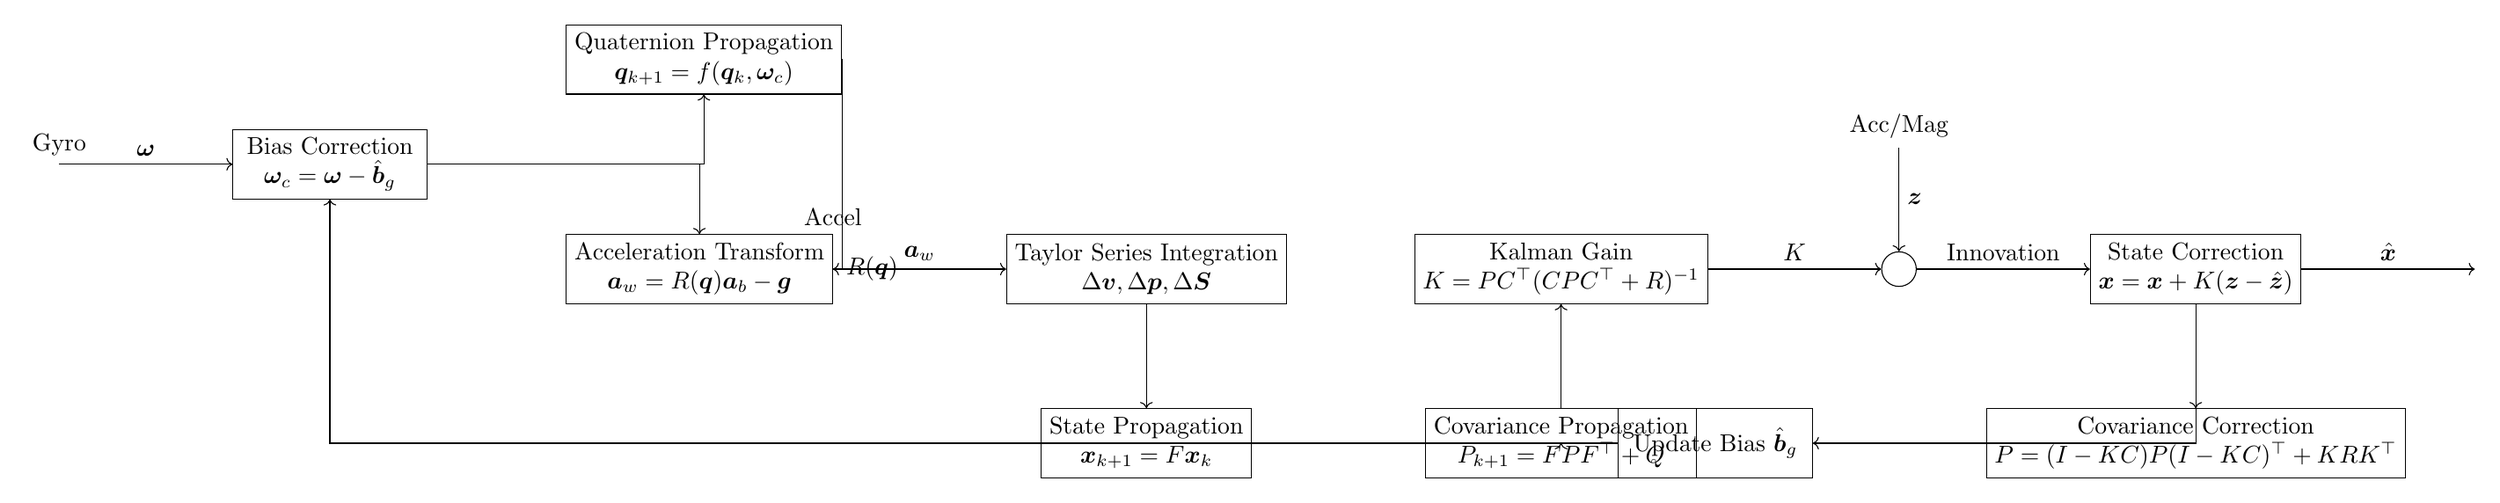
\begin{tikzpicture}[
    node distance=1.5cm and 2.5cm,
    block/.style={rectangle, draw, minimum height=1cm, minimum width=2.8cm, align=center},
    sum/.style={circle, draw, minimum size=0.5cm},
    input/.style={coordinate},
    output/.style={coordinate}
]
% Nodes
\node [input] (gyro-in) {};
\node [block, right=of gyro-in] (bias-correction) {Bias Correction\\$\bm{\omega}_c = \bm{\omega} - \hat{\bm{b}}_g$};
\node [block, above right=0.5cm and 2cm of bias-correction] (q-propagate) {Quaternion Propagation\\$\bm{q}_{k+1} = f(\bm{q}_k, \bm{\omega}_c)$};
\node [block, below right=0.5cm and 2cm of bias-correction] (acc-transform) {Acceleration Transform\\$\bm{a}_w = R(\bm{q})\bm{a}_b - \bm{g}$};
\node [block, right=of acc-transform] (integrators) {Taylor Series Integration\\$\Delta\bm{v}, \Delta\bm{p}, \Delta\bm{S}$};
\node [block, below=of integrators] (state-update) {State Propagation\\$\bm{x}_{k+1} = F\bm{x}_k$};
\node [block, right=of state-update] (cov-update) {Covariance Propagation\\$P_{k+1} = F P F^\top + Q$};
\node [block, above=of cov-update] (k-gain) {Kalman Gain\\$K = PC^\top(CPC^\top + R)^{-1}$};
\node [sum, right=of k-gain] (sum-meas) {};
\node [input, above=of sum-meas] (meas-in) {};
\node [block, right=of sum-meas] (state-correct) {State Correction\\$\bm{x} = \bm{x} + K(\bm{z} - \hat{\bm{z}})$};
\node [block, below=of state-correct] (cov-correct) {Covariance Correction\\$P = (I-KC)P(I-KC)^\top + KRK^\top$};
\node [block, left=of cov-correct] (bias-update) {Update Bias $\hat{\bm{b}}_g$};
\node [output, right=of state-correct] (out) {};

% Arrows
\draw[->] (gyro-in) -- node[above] {$\bm{\omega}$} (bias-correction);
\draw[->] (bias-correction) -| (q-propagate);
\draw[->] (bias-correction) -| (acc-transform);
\draw[->] (q-propagate) -- ++ (2,0) node[input] (rot-out) {} |- node[near end, right] {$R(\bm{q})$} (acc-transform);
\draw[->] (acc-transform) -- node[above] {$\bm{a}_w$} (integrators);
\draw[->] (integrators) -- (state-update);
\draw[->] (state-update) -| (cov-update);
\draw[->] (cov-update) -- (k-gain);
\draw[->] (k-gain) -- node[above] {$K$} (sum-meas);
\draw[->] (meas-in) -- node[right] {$\bm{z}$} (sum-meas);
\draw[->] (sum-meas) -- node[above] {Innovation} (state-correct);
\draw[->] (state-correct) -- node[above] {$\hat{\bm{x}}$} (out);
\draw[->] (state-correct) -- (cov-correct);
\draw[->] (state-correct) |- (bias-update);
\draw[->] (bias-update) -| (bias-correction);

% Labels
\node [above] at (gyro-in.north) {Gyro};
\node [above] at (meas-in.north) {Acc/Mag};
\node [above] at (acc-transform.north east) {Accel};
\end{tikzpicture}
\caption{Data flow diagram of the extended Kalman filter, showing the interaction between the quaternion propagation, state prediction, and measurement update steps.}
\label{fig:dataflow}
\end{figure}

\section{Implementation Overview}
\label{sec:implementation}

The provided C++ implementation is a template class \texttt{Kalman3D\_Wave<T, with\_bias>} designed for efficiency and flexibility on embedded platforms, leveraging the Eigen library for linear algebra.

\subsection{Key Data Structures}
\begin{itemize}
    \item \texttt{qref}: The reference quaternion (\texttt{Eigen::Quaternion<T>}).
    \item \texttt{xext}: The full error state vector (\texttt{Eigen::Matrix<T, NX, 1>}).
    \item \texttt{Pext}: The full error state covariance matrix (\texttt{Eigen::Matrix<T, NX, NX>}).
    \item \texttt{Pbase}: A mirror of the top-left $6\times6$ or $3\times3$ block of \texttt{Pext}, maintained for compatibility with the original MEKF structure.
\end{itemize}

\subsection{Main Algorithmic Steps}
The flow of the algorithm, also depicted in \cref{fig:dataflow}, is as follows:
\begin{enumerate}
    \item \textbf{Initialization:} The filter is initialized from accelerometer and magnetometer data using the \texttt{initialize\_from\_acc\_mag} method, which aligns the reference quaternion with the local gravity and magnetic field.
    \item \textbf{Time Update (\texttt{time\_update}):}
    \begin{enumerate}
        \item Correct gyro reading for estimated bias.
        \item Propagate the reference quaternion.
        \item Calculate world-frame acceleration.
        \item Propagate the linear states $\bm{v}, \bm{p}, \bm{S}$ using the Taylor series.
        \item Assemble the extended Jacobian $F$ and process noise $Q$.
        \item Propagate the covariance matrix: $P_{k+1} = F P_k F^\top + Q$.
    \end{enumerate}
    \item \textbf{Measurement Update:} Can be performed using both sensors (\texttt{measurement\_update}), or individually (\texttt{measurement\_update\_acc\_only}, \texttt{measurement\_update\_mag\_only}).
    \begin{enumerate}
        \item Calculate the predicted sensor measurements.
        \item Form the measurement Jacobian $C$.
        \item Compute the Kalman gain $K$.
        \item Update the state vector and covariance matrix (using the Joseph form for numerical stability).
        \item Apply the estimated attitude error to the reference quaternion and reset the error state.
    \end{enumerate}
    \item \textbf{Drift Correction (\texttt{applyIntegralZeroPseudoMeas}):} This optional step can be called after the time update. It performs a measurement update step using the pseudo-measurement $H_S$ and $R_S$ to constrain the integral state.
\end{enumerate}

\section{Conclusion}
\label{sec:conclusion}
We have presented a comprehensive extension of the MEKF for integrated attitude and wave motion estimation. By augmenting the state vector to include velocity, position, and a novel integral state, and by carefully deriving the corresponding system Jacobian and process noise, the filter provides a mathematically sound framework for fusing IMU data. The integral state pseudo-measurement offers an effective and tunable method for mitigating the inherent drift of inertial navigation, making the filter particularly suitable for applications like wave motion tracking. The provided object-oriented C++ implementation offers a practical and efficient tool for researchers and engineers working in this domain.

\bibliographystyle{ieeetr}
\begin{thebibliography}{9}
\bibitem{crassidis2007survey}
J. L. Crassidis and F. L. Markley.
\newblock Survey of Nonlinear Attitude Estimation Methods.
\newblock \emph{Journal of Guidance, Control, and Dynamics}, 30(1):12--28, 2007.

\bibitem{markley2003attitude}
F. L. Markley.
\newblock Attitude Error Representations for Kalman Filtering.
\newblock \emph{Journal of Guidance, Control, and Dynamics}, 26(2):311–317, 2003.

\bibitem{farrell2008aided}
A. Farrell.
\newblock \emph{Aided Navigation: GPS with High Rate Sensors}.
\newblock McGraw-Hill, 2008.

\bibitem{trawny2005indirect}
N. Trawny and S. I. Roumeliotis.
\newblock Indirect Kalman Filter for 3D Attitude Estimation.
\newblock Technical Report, University of Minnesota, 2005.
\end{thebibliography}

\end{document}
